\section{Theory}
% \newcommand{\na}{$^{22}$Na}
% \newcommand{\ne}{$^{22}$Ne}

\subsection{$^{22}$Na Decay}

\begin{figure}
    \centering
    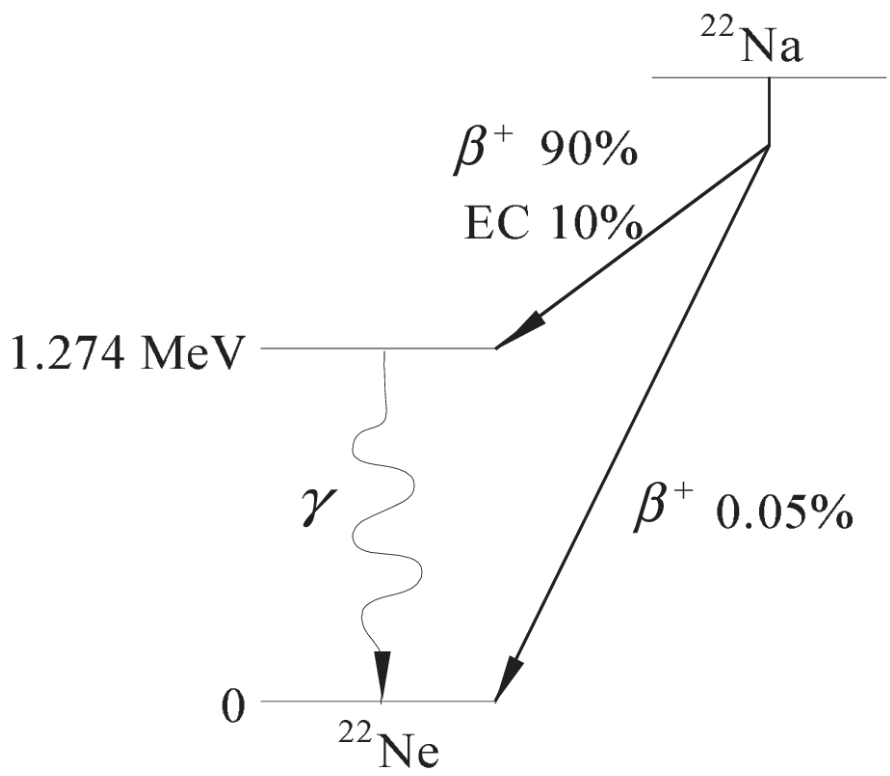
\includegraphics[width=0.6\columnwidth]{images/expt.png}
    \caption{$^{22}$Na decay summarised}
    \label{expt}
\end{figure}

$^{22}$Na radioactively deacys into an excited state of 
$^{22}$Ne either by emission of a positron (with 90\%) probability or by electron capture (10\% probability). The excited $^{22}$Ne nucleus decaus with a mean life of $3\times 10^{-12}$ s to the ground state with the emission of a 1.274 MeV gamma photon (Fig. \ref{expt}).

Positrons are emitted with a range of kinetic energies upto about 0.5 MeV. They lose this energy within nanoseconds of release in the material sorrounding the source and when the reach atomic energies (eV), capture an electron to form positronium -- a hydrogen like `atom', which decays by the annihilation of the $e^+$ and $e^-$ into two gamma photons. By energy conservation, the energy of these photons must equal the net rest energy of the positronium, hence they will each have an energy of 0.511 MeV (ignoring the binding energy $\sim$ a few eV). By momentum conservation, the net momentum of the two photons must equal the initial momentum of the positronium. Since in its rest frame there is no inital momentum, the two annihilation gamma photons must have equal and opposite momentum in that frame. This allows for simultaneous detection in two scintillation detectors placed on both sides of the sample, i.e. $\gamma-\gamma$ coincidence.

However it is to be noted that in a situation where the positronium is not at rest, depending on the direction of the initial positronium momentum relative to the gamma emission direction, the transformation to the lab frame may give gamma energies that are not 0.511 MeV and/or produce gammas that are not emitted exactly 180$^\circ$ apart.

\subsection{Coincidence Rate}

The nuclear decay rate (number of nuclear decays per second) is $\Gamma_n = \alpha \cdot 3.7 \times 10^{10}$ decays/sec/curie, where $\alpha$ is the source activity in curies. 90\% of the time, the nuclear decay proceeds by $\beta^+$ emission, and these always annihilate with an electron to produce two 0.511 MeV gammas. Thus the rate of emission of 0.511 MeV gammas is $0.9 \cdot 2 \cdot \Gamma_n = 1.8\Gamma_n$. These gammas are emitted uniformly (in oppositely directed pairs) from the source. 

Thus at a distance $R$ from the source they are spread out over an area $4\pi R^2$ and the flux $\Phi$ (number per unit area per second) will be,

\begin{align}
    4\pi R^2\Phi = 1.8\Gamma_n 
\end{align}

The fraction of 0.511 MeV gammas which get through the lead shielding will  is expected to be on the order of 20\% and is expressed by the symbol $\kappa$. Hence, the rate $Q$ of 0.511 MeV gammas striking the face of the scintillator can be calculated as,

\begin{align}
    Q = \Phi[A_a+\kappa(A_s-A_a)]
\end{align}

Here, $A_a = \pi r_a^2$ is the area of the aperture and $A_s=\pi r_s^2$ is the area of the scintillator.

% =========================================================================
\section{Experimental Setup}

\subsection*{Apparatus}

\begin{figure}[H]
    \centering
    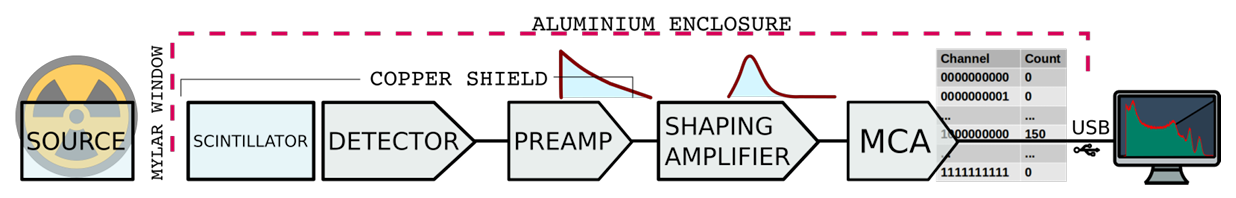
\includegraphics[width=1\columnwidth]{images/setup.png}
    \caption{A flow diagram of the experimental setup}
    \label{setup}
\end{figure}

\begin{enumerate}
    \item $^{22}$Na source
    \item Two scintillation detectors
    \item Gamma ray spectroscopy setup, with Multiple Channel Analyser (MCA)
    \item Software (\verb|CNSPEC|) and computer for analysis\\
\end{enumerate}

The experimental setup is that of a gamma ray spectroscope with multiple channel analyser with two scintillation detectors (Fig. \ref{setup}, \ref{instr}). The detector is made of an 8mm diameter entrance window coated in aluminium to block visible light. Inside, a PN junction coupled in reverse bias mode is mated to a scintillator that measures 10mm $\times$ 10mm $\times$ 8mm. The scintillator is made of NaI with Thorium doping that emits photns with the same energy as the gamma ray's descent. The scintillation photons are transformed into an equivant amount of electron-hole pairs in the depeletion area of the PN junction. An event in the photopeak area transforms into a charge pulse in the PN junction. The preamplifier converts it into a matching output voltage (of the range 0 to 3.3V) and the shaping amplifier then generates a pulse with a Gaussian form. The signal enters the MCA and a spectrum is produced with 10 bit resolution. \verb|CNSPEC| software is then used for data analysis \cite{Jithin_Sastri_2018}.

\begin{figure}[H]
    \centering
    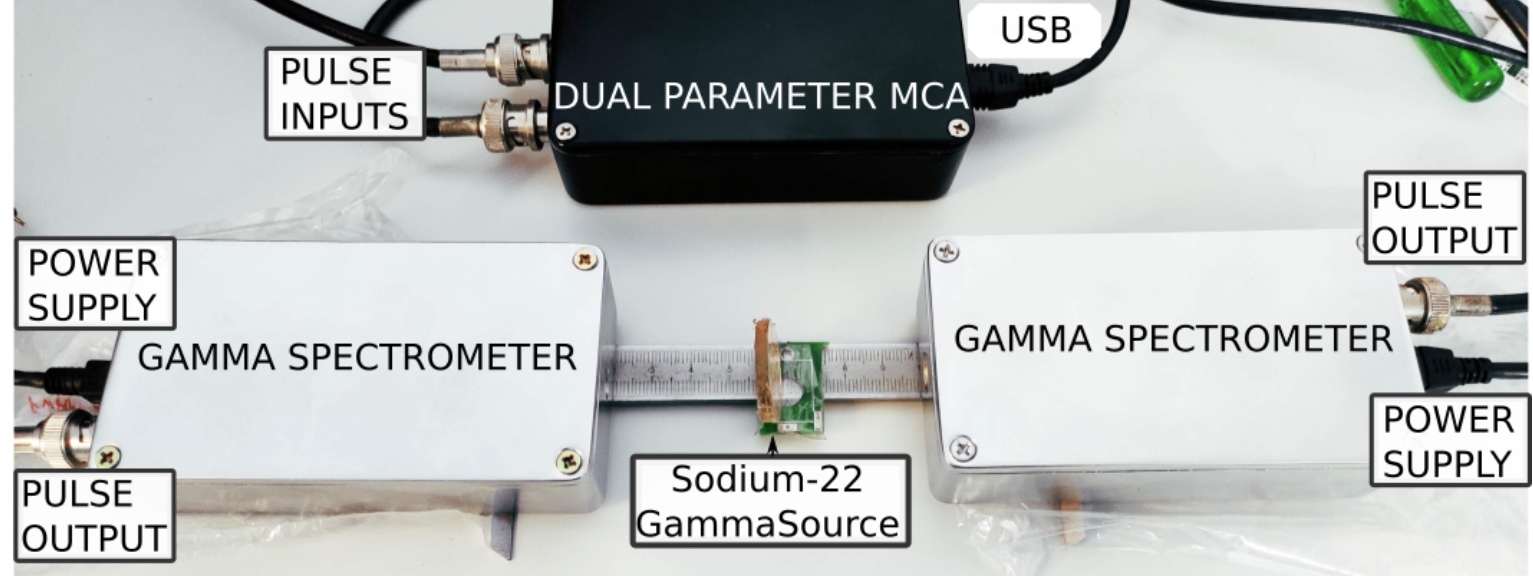
\includegraphics[width=1\columnwidth]{images/instr.png}
    \caption{The experimental setup, composed of two gamma spectrometers placed with a $^{22}$Na source in the middle. Data acquisition is carried out by the Multiple Channel Analyser}
    \label{instr}
\end{figure}

